\part{Ordinary differential equations I - Explicit methods}
\section{Introduction}
\subsection*{General}
\begin{frame}[label=contents_ode1]
  \frametitle{Today's outline}
  \mode<beamer>{
    \only<1>{\tableofcontents}
  }
  \only<2>{\tableofcontents[currentsection]}
\end{frame}
 
\begin{frame}
  \frametitle{Overview}
    \begin{block}{Ordinary differential equations}
      An equation containing a function of one independent variable and its derivatives, in contrast to a \emph{partial differential equation}, which contains derivatives with respect to more independent variables.
    \end{block}
    \pause
  \begin{block}{Main question}
  How to solve 
  \[
    \frac{d\vec{y}}{dx} = f(\vec{y}(x),x) \quad \text{with} \quad \vec{y}(x=0) = \vec{y}_0
  \]
  accurately and efficiently?
  \end{block}
\end{frame}

\begin{frame}
  \frametitle{What is an ODE?}
  \begin{itemize}
    \item Algebraic equation:
    \[
      f(y(x),x) = 0 \qquad \text{e.g.} \, -\ln(K_{eq})=(1-\zeta)
    \]
    \item First order ODE:
    \[
      f\left(\frac{dy}{dx}(x),y(x),x\right) = 0 \quad \text{e.g.} \, \frac{dc}{dt} = -kc^n
    \]
    \item Second order ODE:
    \[
      f\left(\frac{d^2y}{dx^2}(x),\frac{dy}{dx}(x),y(x),x \right) = 0 \quad \text{e.g.} \quad \mathcal{D}\frac{d^2c}{dx^2}= - \frac{kc}{1+Kc}
    \]
  \end{itemize}
\end{frame}

\begin{frame}
  \frametitle{About second order ODEs}
  Very often a second order ODE can be rewritten into a system of first order ODEs (whether it is handy depends on the boundary conditions!)
  \vskip1em
  \pause
  \mode<beamer>{
  \only<1-2>{
  \begin{block}{Example}
  Recall:
  \[
    \mathcal{D}\frac{d^2c}{dx^2}= - \frac{kc}{1+Kc}
  \]
  Define $y = -\mathcal{D} \frac{dc}{dx}$, then $\frac{dy}{dx}=\frac{kc}{1+Kc}$, thus solve system:
  \begin{align*}
    \frac{dc}{dx} &= -\frac{1}{\mathcal{D}}y \\
    \frac{dy}{dx} &= \frac{kc}{1+Kc}
  \end{align*}
  \end{block}}}
  \only<3>{
  \begin{block}{More general}
  Consider the second order ODE:
  \[
    \frac{d^2y}{dx^2} + q(x)\frac{dy}{dx} = r(x)
  \]
  Now define and solve using $z$ as a new variable:
  \begin{align*}
    \frac{dy}{dx} &= z(x) \\
    \frac{dz}{dx} &= r(x) - q(x)z(x)
  \end{align*}
  \end{block}}
  \vskip1em
  \pause
\end{frame}

\begin{frame}[label=ivpbvp]
  \frametitle{Importance of boundary conditions}
  \footnotesize\selectfont
  The nature of boundary conditions determines the appropriate numerical method. Classification into 2 main categories:
  \begin{itemize}
    \item \emph{Initial value problems (IVP)} \\
    We know the values of all $y_i$ at some starting position $x_s$, and it is desired to find the values of $y_i$ at some final point $x_f$. \vskip1em
    \begin{center}
      \begin{tikzpicture}[scale=5]
        \node[] (y1s) at (0,0.1) {$y_{1,s}$};
        \node[] (y1f) at (1,0.1) {\color{scharlaken}$y_{1,f}$};
        \node[] (y2s) at (0,0) {$y_{2,s}$};
        \node[] (y2f) at (1,0) {\color{scharlaken}$y_{2,f}$};
        \node[fdot] (xs) at (0,-0.1) {};
        \node[fdot] (xf) at (1,-0.1) {};
        \node[anchor=north] at (xs.south) {$x_s$};
        \node[anchor=north] at (xf.south) {$x_f$};
        \draw[line] (xs) -- (xf);
        \draw[line,->,densely dashed] (0.1,0.05) -- node[midway,above] {``Marching''} (0.9,0.05);
      \end{tikzpicture}
    \end{center}
    \item \emph{Boundary value problems (BVP)} \\
    Boundary conditions are specified at more than one $x$. Typically, some of the BC are specified at $x_s$ and the remainder at $x_f$. \vskip1em
    \centering
    \begin{tikzpicture}[scale=5]
      \node[] (y1s) at (0,0.1) {$y_{1,s}$};
\node[] (y1f) at (1,0.1) {\color{scharlaken}$y_{1,f}$};
\node[] (y2s) at (0,0) {\color{scharlaken}$y_{2,s}$};
\node[] (y2f) at (1,0) {$y_{2,f}$};
\node[fdot] (xs) at (0,-0.1) {};
\node[fdot] (xf) at (1,-0.1) {};
\node[anchor=north] at (xs.south) {$x_s$};
\node[anchor=north] at (xf.south) {$x_f$};
\draw[line] (xs) -- (xf);
\draw[line,->,densely dashed] (0.1,0.05) -- node[midway,above] {``Shooting''} (0.9,0.05);

\coordinate[] (b) at ($(y1f)!0.5!(y2f) + (0.1,0) $) {};
\coordinate[right of=b] (c1) {};
\coordinate[below=1.4cm] (c2) at (c1)  {};
%       \coordinate[below of=1cm] at (c2) (c5) {};

\coordinate[] (s) at ($(y1s)!0.5!(y2s) - (0.1,0) $) {};
\coordinate[left of=s] (c3) {};
\coordinate[below=1.4cm] (c4) at (c3)  {};
%       \coordinate[below of=c4] (c6) {};

%       \node[] (b) at ($(y1f)!0.5!(y2f)$) {};
\draw[line,->,densely dashed,draw=tuegreen,rounded corners=10pt] (b) -- (c1) -- (c2) -- (c4) -- (c3) -- (s);
%       \draw[line,densely dashed,draw=tuegreen] (y2f) to [controls=(1,-0.2) and +(-0.1,-0.2)] (y2s);
    \end{tikzpicture}
  \end{itemize}
\end{frame}

\begin{frame}
  \frametitle{Overview}
  Initial value problems:
  \begin{itemize}
    \colorize<2> \item Explicit methods
    \begin{itemize}
      \colorize<2> \item First order: forward Euler
      \colorize<2> \item Second order: improved Euler (RK2)
      \colorize<2> \item Fourth order: Runge-Kutta 4 (RK4)
      \colorize<2> \item Step size control
    \end{itemize}
    \colorize<3> \item Implicit methods
    \begin{itemize}
      \colorize<3> \item First order: backward Euler
      \colorize<3> \item Second order: midpoint rule
    \end{itemize}
  \end{itemize}
  \onslide<4>{
  Boundary value problems
  \begin{itemize}
    \colorize<4> \item Shooting method
  \end{itemize}
  }
\end{frame}

\section{Euler's method}
\againframe<2>{contents_ode1}
\subsection{Forward Euler}
\begin{frame}
  \frametitle{Euler's method}
  Consider the following single initial value problem:
  \[
    \frac{dc}{dt} = f(c(t),t) \quad \text{with} \quad c(t=0)=c_0 \quad \text{(initial value problem)}
  \]
  \pause
  Easiest solution algorithm: Euler's method, derived here via Taylor series expansion:
  \[
    c(t_0 + \Delta t) \approx c(t_0) + \left.\frac{dc}{dt}\right|_{t_0}\Delta t + \frac{1}{2} \left.\frac{d^2c}{dt^2}\right|_{t_0} \left(\Delta t\right) ^2 + \mathcal{O}{(\Delta t^3)}
  \]
  \pause
  Neglect terms with higher order than two: $\left. \frac{dc}{dt}\right|_{t_0} = \frac{c(t_0 + \Delta t) - c(t_0)}{\Delta t}$
  Substitution: 
  \[
    \frac{c(t_0 + \Delta t) - c(t_0)}{\Delta t} = f(c_0,t_0)\Rightarrow c(t_0+\Delta t) = c(t_0) + \Delta t f(c_0,t_0) 
  \]
\end{frame}

\begin{frame}[t,fragile]
  \frametitle{Euler's method: graphical example}
  \[
    \frac{c(t_0 + \Delta t) - c(t_0)}{\Delta t} = f(c_0,t_0)\Rightarrow c(t_0+\Delta t) = c(t_0) + \Delta t f(c_0,t_0) 
  \]
  \vskip1em
   \begin{tikzpicture}
      \begin{axis}[every axis/.append style={font=\footnotesize},
      width=\columnwidth, height=5.5cm,
      xmin=0,xmax=4,ymin=0,ymax=4,
      xtick={1,2,3},ytick={1,2,2.5},
      axis x line=middle,axis y line=middle,
      xlabel=$t$,xticklabels={$t_0$,$\Delta t$,$2\Delta t$},
      ylabel=$c(t)$,yticklabels={$c_0$,$c_1$,$c_2$},tick align=outside,ymajorgrids=true,major grid style={dashed}]
 
    \addplot[graph,quiver={u=\thisrow{u},v=\thisrow{v},scale arrows=0.4},-stealth']
      table {
      x y u v
      1 1 1 1
      2 2 1 0.5
      };
      \addplot[graph,sharp plot,densely dashed,mark=*,mark options={solid,fill=scharlaken},mark size=1.7pt,nodes near coords={\coordindex}]
      table {
      x y
      1 1
      2 2
      3 2.5
      };
      \node[black] at (axis cs:1.4,0.9) {$\left.\frac{dc}{dt}\right|_{t_0}$};
      \node[black] at (axis cs:2.4,1.8) {$\left.\frac{dc}{dt}\right|_{\Delta t}$};
%       \node[black] at (axis cs:2.1,0.5) {$k_1$};
    \end{axis}
  \end{tikzpicture}
\end{frame}

\begin{frame}
  \frametitle{Euler's method - solution method}
    \begin{tikzpicture}[]
    %draw horizontal line   
    \draw (0,0) -- (6,0);
    \draw[decorate,decoration=triangles] (6.2,0) -- (8.0,0);
    \draw (8,0) -- (10,0);

    %draw vertical lines
    \foreach \x in {0,2,4,6,8,10}
      \draw (\x cm,3pt) -- (\x cm,-3pt);

    %draw nodes
    \draw (0,0) node[below=3pt] {$ t=0 $} node[above=3pt] {$ 1 $};
    \draw (2,0) node[below=3pt] {$ \Delta t $} node[above=3pt] {$ 2 $};
    \draw (4,0) node[below=3pt] {$ 2\Delta t $} node[above=3pt] {$ 3 $};
    \draw (6,0) node[below=3pt] {$ 3\Delta t $} node[above=3pt] {$ 4 $};
    \draw (8,0) node[below=3pt] {$ t_\mathrm{end}-\Delta t $} node[above=3pt] {$ n-1 $};
    \draw (10,0) node[below=3pt] {$ t_\mathrm{end} $} node[above=3pt] {$ n $};
    
    \onslide<1>{
      \draw (0,-1.5) node[above=1pt] {$c_0$};
    }
    \onslide<2>{
      \draw (0,-1.5) node[above=1pt] {$c(t)$};
      \draw (2,-1.5) node[above=1pt] {$c(t+\Delta t)$};
    }
    \onslide<3>{
      \draw (2,-1.5) node[above=1pt] {$c(t)$};
      \draw (4,-1.5) node[above=1pt] {$c(t+\Delta t)$};
    }
    \onslide<4>{
      \draw (4,-1.5) node[above=1pt] {$c(t)$};
      \draw (6,-1.5) node[above=1pt] {$c(t+\Delta t)$};
    }
   \end{tikzpicture}
   \vskip1em
  Start with $t = t_0$, $c=c_0$, then calculate at discrete points in time: $c(t_1 = t_0 + \Delta t) = c(t_0) + \Delta t f(c_0,t_0)$. 
  \onslide<5>{
  \vskip1em
  \tikz{\node[emphblock,text width=\textwidth] {
  Pseudo-code Euler's method: $ \frac{dy}{dx} = f(x,y) \quad \text{and} \quad y(x_0) = y_0$.
  \begin{enumerate}
    \item Initialize variables, functions; set $h = \frac{x_1 - x_0}{N}$
    \item Set $x = x_0$, $y = y_0$
    \item While $x<x_\text{end}$ do\\
    $ \displaystyle x_{i+1} = x_i + h; \quad y_{i+1} = y_i + h f(x_i,y_i)$
  \end{enumerate}
  };}
  }
\end{frame}


\begin{frame}
  \frametitle{Euler's method - example}
  First order reaction in a batch reactor:
  \[
    \frac{dc}{dt} = -kc \quad \text{with} \quad c(t=0) = 1\, \si{\mole\per\cubic\meter}, \quad k = 1\, \si{s^{-1}}, \quad t_\text{end} = 2\, \si{\second}
  \]
  \pause
  \footnotesize\selectfont
  \begin{longtable}{p{0.3\textwidth}p{0.5\textwidth}}
  \hline
    Time [\si{\second}] & Concentration [\si{\mole\per\cubic\meter}] \\ \hline
    $t_0 = 0$                                 & $c_0 = 1.00$ \\
    $\begin{aligned}t_1 &= t_0 + \Delta t\\ &= 0 + 0.1 = 0.1\end{aligned}$    & $\begin{aligned}c_1 &= c_0 + \Delta t \cdot (-kc_0) \\ &= 1 + 0.1 \cdot (-1 \cdot 1) = 0.9\end{aligned}$ \\
    $\begin{aligned}t_2 &= t_1 + \Delta t\\ &= 0.1 + 0.1 = 0.2\end{aligned}$  & $\begin{aligned}c_2 &= c_1 + \Delta t \cdot (-kc_1)\\ &= 0.9 + 0.1 \cdot (-1 \cdot 0.9) = 0.81\end{aligned}$ \\ 
    $\begin{aligned} t_3 &= t_2 + \Delta t \\ &= 0.2 + 0.1 = 0.3\end{aligned}$  & $\begin{aligned}c_3 &= c_2 + \Delta t \cdot (-kc_2)\\ &= 0.81 + 0.1 \cdot (-1 \cdot 0.81) = 0.729 \end{aligned}$ \\ 
    \centering$\ldots$                                  & $\quad \quad \quad \quad \ldots$ \\
    $t_{i+1} = t_i + \Delta t$                & $c_{i+1} = c_i + \Delta t \cdot (-k c_i) $ \\
    \centering$\ldots$ & $\quad \quad \quad \quad \ldots$ \\
    $t_{20} = 2.0 $ & $c_{20} = c_{19} + \Delta t \cdot (-k c_{19}) = 0.121577$ \\
    \hline
  \end{longtable}
\end{frame}

\begin{frame}
  \frametitle{Euler's method - example}
  %   Accuracy: Results are shown for $N=20,4-,80,\ldots,320$ using $k = 1 \si{s^{-1}$
  \begin{center}
    \begin{tikzpicture}
      \begin{axis}[every axis/.append style={font=\footnotesize},
        width=\textwidth, height=7cm,     % size of the image
    grid = major,
    grid style={dashed, gray!30},
    xmin=0,     % start the diagram at this x-coordinate
    xmax=2,    % end   the diagram at this x-coordinate
    ymin=0,     % start the diagram at this y-coordinate
    ymax=1,   % end   the diagram at this y-coordinate
    xtick={0,0.2,...,2},
    ytick={0,0.2,...,1},
    axis background/.style={fill=white},
    axis x line=middle,
    axis y line=middle,
    ylabel style={at={(ticklabel* cs:1.05)},anchor=south west},
    ylabel=$c$ (\si{\mole\per\cubic\meter}),
    xlabel=$t$ (\si{\second}),
    tick align=outside,
    legend style={draw=none,fill=none,font=\tiny,at={(0.5,1.0)},anchor=south},
    legend columns=5
    ]
    
    \addplot[graph,mark=x] table [id=EE_20]{data/ODE_EulerExpl_20.dat};  \addlegendentry{20 points}
      \only<2->{\addplot[graph,draw=tueyellow] table [id=EE_20]{data/ODE_EulerExpl_40.dat}; } \addlegendentry{40 points}
      \only<3->{\addplot[graph,draw=tuesteel] table [id=EE_20]{data/ODE_EulerExpl_80.dat}; } \addlegendentry{80 points}
      \only<4->{\addplot[graph,draw=tuegreen] table [id=EE_20]{data/ODE_EulerExpl_160.dat};} \addlegendentry{160 points}
      \only<5->{\addplot[graph,draw=tuepurple] table [id=EE_20]{data/ODE_EulerExpl_320.dat};} \addlegendentry{320 points}
    \end{axis}
  \end{tikzpicture}
  \end{center}
\end{frame}

\begin{frame}<handout:0|beamer:1->[fragile]
  \frametitle{Euler's method - implementation}
  A basic function of Euler's method is given in \lstinline$ode_scalar_explicit.py$:
  \begin{lstlisting}
def euler_basic(func, c0, t0, tend, n=100):
    dt = (tend - t0)/n
    t,c = t0, c0
    print(f"t: {t:1.2f}, c: {c:1.6f}")
    for i in range(n):
        k1 = func(c, t)
        t += dt
        c += dt*k1
        print(f"t: {t:1.2f}, c: {c:.6f}")
  \end{lstlisting}
  \pause
  \begin{columns}
    \column{0.65\textwidth}
    \vspace*{-2em}\\
  We define the ODE function to be solved, e.g. $\frac{dc}{dt} = -kc$ with $k=1$, and pass it as an argument to \lstinline$euler_basic$:
  \begin{lstlisting}
def first_order_react(c,t):
    dcdt = -c
    return dcdt

euler_basic(first_order_react, 1, 0, 2, 100)
  \end{lstlisting}
    \column{0.3\textwidth}
      \begin{lstlisting}[style=PyOutput]
t: 0.00, c: 1.000000
t: 0.20, c: 0.800000
t: 0.40, c: 0.640000
t: 0.60, c: 0.512000
t: 0.80, c: 0.409600
t: 1.00, c: 0.327680
t: 1.20, c: 0.262144
t: 1.40, c: 0.209715
t: 1.60, c: 0.167772
t: 1.80, c: 0.134218
t: 2.00, c: 0.107374
      \end{lstlisting}
  \end{columns}
\end{frame}

\begin{frame}<handout:0|beamer:1->[fragile]
  \frametitle{Euler's method - implementation}
  By storing the intermediate results we can return the results for post processing:
  \begin{lstlisting}
import numpy as np
def euler(func, c0, t0, tend, n=100):
    dt = (tend - t0)/n
    t = np.linspace(t0,tend,n+1)
    c = np.zeros(n+1)
    c[0] = c0
    for i in range(n):
        k1 = func(c[i], t[i]) 
        c[i+1] = c[i] + dt*k1
    return c,t
  \end{lstlisting}
  \pause
  The function \lstinline$euler$ can be imported from \lstinline$ode_scalar_explicit.py$:
  \begin{lstlisting}
from ode_scalar_explicit import euler
c, t = euler(first_order_react, 1, 0, 2, 100)
print(np.vstack([t,c]).T)
  \end{lstlisting}
  Alternatively, we can pass a \emph{lambda function} in-place:
  \begin{lstlisting}
c, t = euler(lambda c, t: -1.0*c, 1, 0, 2, 100)
  \end{lstlisting} 
\end{frame}

{\nologo
\begin{frame}
  \frametitle{Problems with Euler's method}
  The question is: What step size, or how many steps to use?
  \begin{enumerate}
    \item \emph{Accuracy}  $\Rightarrow$ need information on numerical error!
    \item \emph{Stability} $\Rightarrow$ need information on stability limits!
  \end{enumerate}
  \vskip1em

  \begin{columns}
    \column{0.5\textwidth}
    \begin{tikzpicture}
      \begin{axis}[every axis/.append style={font=\tiny},
      width=\columnwidth, height=5.5cm,     % size of the image
      grid = major,
      grid style={dashed, gray!30},
      xmin=0,     % start the diagram at this x-coordinate
      xmax=2,    % end   the diagram at this x-coordinate
      ymin=0,     % start the diagram at this y-coordinate
      ymax=1,   % end   the diagram at this y-coordinate
      xtick={0,0.5,...,2},
      ytick={0,0.25,...,1},
%       axis background/.style={fill=white},
%       axis x line=middle,
%       axis y line=middle,
      xlabel style={at={(ticklabel* cs:1.1)},anchor=south},
      xlabel=$t$ (\si{\second}),
      ylabel style={at={(yticklabel* cs:0.7)},anchor=north,left=7mm},
      ylabel=$c$ (\si{\mole\per\cubic\meter}),
      tick align=outside,
      legend style={draw=none,fill=none,font=\tiny,at={(0.5,-0.1)},anchor=north},
      legend columns=3
      ]

	\addplot[graph] table [id=EE_20]{data/ODE_EulerExpl_20.dat}; \addlegendentry{$N=20$}
	\addplot[graph,draw=tueyellow] table [id=EE_20]{data/ODE_EulerExpl_40.dat}; \addlegendentry{$N=40$}
	\addplot[graph,draw=tuesteel] table [id=EE_20]{data/ODE_EulerExpl_80.dat};  \addlegendentry{$N=80$}
	\addplot[graph,draw=tuegreen] table [id=EE_20]{data/ODE_EulerExpl_160.dat}; \addlegendentry{$N=160$}
	\addplot[graph,draw=tuepurple] table [id=EE_20]{data/ODE_EulerExpl_320.dat}; \addlegendentry{$N=320$}
      \end{axis}
    \end{tikzpicture}
     \centering Reaction rate: $k = 1$ \si{s^{-1}}
    \column{0.5\textwidth}
    \begin{tikzpicture}
      \begin{axis}[every axis/.append style={font=\tiny},
      width=\columnwidth, height=5.5cm,     % size of the image
      grid = major,
      grid style={dashed, gray!30},
      xmin=0,     % start the diagram at this x-coordinate
      xmax=0.25,    % end   the diagram at this x-coordinate
      ymin=-5,     % start the diagram at this y-coordinate
      ymax=5,   % end   the diagram at this y-coordinate
      restrict y to domain*=-300:300,
      xtick={0,0.05,...,0.25},
      ytick={-5,-2.5,...,5},
%       axis background/.style={fill=white},
% %       axis x line=middle,
%       axis y line=middle,
      xlabel style={at={(ticklabel* cs:1.1)},anchor=south},
      xlabel=$t$ (\si{\second}),
      ylabel style={at={(yticklabel* cs:0.7)},anchor=north,left=7mm},
      ylabel=$c$ (\si{\mole\per\cubic\meter}),
      tick align=outside,
      legend style={draw=none,fill=none,font=\tiny,at={(0.5,-0.1)},anchor=north},
      legend columns=3
      ]

	\addplot[graph,sharp plot,mark=+,mark size=1.3pt] table [id=EE_20]{data/ODE_Euler2Expl_20.dat}; \addlegendentry{$N=20$}
	\addplot[graph,sharp plot,draw=tueyellow,mark=x,mark size=1.3pt] table [id=EE_20]{data/ODE_Euler2Expl_40.dat}; \addlegendentry{$N=40$}
	\addplot[graph,sharp plot,draw=tuesteel,mark=o,mark size=1.3pt] table [id=EE_20]{data/ODE_Euler2Expl_80.dat};  \addlegendentry{$N=80$}
	\addplot[graph,sharp plot,draw=tuegreen] table [id=EE_20]{data/ODE_Euler2Expl_160.dat}; \addlegendentry{$N=160$}
	\addplot[graph,sharp plot,draw=tuepurple] table [id=EE_20]{data/ODE_Euler2Expl_320.dat}; \addlegendentry{$N=320$}
      \end{axis}
    \end{tikzpicture}
     \centering Reaction rate: $k = 50$ \si{s^{-1}}
  \end{columns}
\end{frame}
}

\begin{frame}
  \frametitle{Accuracy}
  Comparison with analytical solution for $k=1$ \si{s^{-1}}:
  \[
    c(t) = c_0 \exp \left(-kt\right) \Rightarrow \zeta = 1-\exp\left(-kt\right) \Rightarrow \zeta_\text{analytical} = 0.864665
  \]
  \begin{columns}[T]
    \column{0.5\textwidth}
      \begin{longtable}{ccc}
      \hline
      $N$ & $\zeta$ & $\frac{\zeta^{}_\text{numerical}-\zeta_\text{analytical}}{\zeta_\text{analytical}}$ \\ \hline
      20  & 0.878423 & 0.015912 \\
      40  & 0.871488 & 0.007891 \\
      80  & 0.868062 & 0.003929 \\
      160 & 0.866360 & 0.001961 \\
      320 & 0.865511 & 0.000979\\
      \hline
    \end{longtable}
  \column{0.5\textwidth}
    \begin{tikzpicture}
      \begin{loglogaxis}[
      width=\columnwidth,height=5cm,
      ylabel style={at={(yticklabel* cs:0.83)},anchor=south,left=13mm},
      xlabel=N,
      ylabel=Relative error,
      log ticks with fixed point,
      xtick={20,40,80,160,320},
      ytick={0.02,0.01,0.005,0.002,0.001}]
      \addplot[graph,draw=tuesteel,mark=o] table {data/ODE_euler_err.dat};
      \end{loglogaxis}
    \end{tikzpicture}
  \end{columns}
\end{frame}

\begin{frame}
  \frametitle{Accuracy}
  \tikz{\node[emphblock,text width=\textwidth] {For Euler's method: Error halves when the number of grid points is doubled, i.e. error is proportional to $\Delta t$: first order method.};}
  \vskip1em
  Error estimate:
  \[
    \left. \frac{dx}{dt}\right|_{t_0} = \frac{x(t_0+\Delta t)-x(t_0)}{\Delta t} + \frac{1}{2} \left.\frac{d^2x}{dt^2}\right|_{t_0} (\Delta t) + \mathcal{O}{(\Delta t)\color{scharlaken}^2}
  \]
  \[
    \frac{x(t_0+\Delta t)-x(t_0)}{\Delta t} = f(x_0,t_0) - \frac{1}{2} \left.\frac{d^2x}{dt^2}\right|_{t_0} (\Delta t) +  \mathcal{O}{(\Delta t)\color{scharlaken}^2}
  \]

\end{frame}

% \subsection{Convergence rate}
% \begin{frame}
%   \frametitle{Errors and convergence rate}
%   \begin{block}{$L_2$ norm (Euclidean norm)}
%     $ \quad \norm{\vec{v}}_2 = \sqrt{v_1^2+v_2^2+\ldots+v_n^2} = \sqrt{\sum_{i=1}^n v_i^2} $
%   \end{block}
%   \begin{block}{$L_\infty$ norm (maximum norm)}
%     $ \quad \norm{\vec{v}}_\infty = \text{max}\left( \abs{v_1},\ldots,\abs{v_n}\right) $
%   \end{block}
%   \begin{block}{Absolute difference}
%     $ \quad \epsilon_\text{abs} = \norm{\vec{y}_\text{numerical} - \vec{y}_\text{analytical}}_{2,\infty} $
%   \end{block}
%   \begin{block}{Relative difference}
%     $ \quad \epsilon_\text{rel} = \frac{\norm{\vec{y}_\text{numerical} - \vec{y}_\text{analytical}}_{2,\infty}}{\norm{\vec{y}_\text{analytical}}_{2,\infty}} $
%   \end{block}
% \end{frame}
% 
\begin{frame}
  \frametitle{Errors and convergence rate}
  \footnotesize\selectfont
   \begin{block}{Convergence rate (or: order of convergence) $r$}
  $\displaystyle \epsilon = \lim_{\Delta x \rightarrow 0} c(\Delta x)^r $
  \end{block}
  \begin{itemize}
    \item A first order method reduces the error by a factor 2 when increasing the number of steps by a factor 2
    \item A second order method reduces the error by a factor 4 when increasing the number of steps by a factor 2
  \end{itemize}
  What to do when there is no analytical solution available?
  \pause
  Compare to calculations with different number of steps: $\epsilon_1 = c(\Delta x_1)^r $ and $\epsilon_2 = c(\Delta x_2)^r $ and solve for $r$: \\ \vfill
  $ \displaystyle
    \frac{\epsilon_2}{\epsilon_1} = \frac{c(\Delta x_2)^r}{c(\Delta x_1)^r} = \left(\frac{\Delta x_2}{\Delta x_1}\right)^r \Rightarrow \log\left( \frac{\epsilon_2}{\epsilon_1}\right) = \log\left( \frac{\Delta x_2}{\Delta x_1}\right)^r $ 
  \vfill
  \tikz{\node[emphblock,text width=\textwidth] {$ \displaystyle
    \Rightarrow r = \frac{\log\left( \frac{\epsilon_2}{\epsilon_1}\right)}{\log\left( \frac{\Delta x_2}{\Delta x_1}\right)} = \frac{\log\left( \frac{\epsilon_2}{\epsilon_1}\right)}{\log\left( \frac{N_1}{N_2}\right)} \quad \text{in the limit of} \quad \Delta x \rightarrow 0 \qquad \text{or} \qquad N \rightarrow \infty $};}
\end{frame}

\section{Rates of convergence}
\againframe<2>{contents_ode1}
\subsection*{Rate of convergence}
\begin{frame}
  \frametitle{Errors and convergence rate}
  \begin{block}{$L_2$ norm (Euclidean norm)}
    $ \quad \norm{\vec{v}}_2 = \sqrt{v_1^2+v_2^2+\ldots+v_n^2} = \sqrt{\sum_{i=1}^n v_i^2} $
  \end{block}
  \begin{block}{$L_\infty$ norm (maximum norm)}
    $ \quad \norm{\vec{v}}_\infty = \text{max}\left( \abs{v_1},\ldots,\abs{v_n}\right) $
  \end{block}
  \begin{block}{Absolute difference}
    $ \quad \epsilon_\text{abs} = \norm{\vec{y}_\text{numerical} - \vec{y}_\text{analytical}}_{2,\infty} $
  \end{block}
  \begin{block}{Relative difference}
    $ \quad \epsilon_\text{rel} = \norm{\frac{\vec{y}_\text{numerical} - \vec{y}_\text{analytical}}{\vec{y}_\text{analytical}}}_{2,\infty} $
  \end{block}
\end{frame}

\begin{frame}
  \frametitle{Errors and convergence rate}
  \footnotesize\selectfont
   \begin{block}{Convergence rate (or: order of convergence) $r$}
  $\displaystyle \epsilon = \lim_{\Delta x \rightarrow 0} c(\Delta x)^r $
  \end{block}
  \begin{itemize}
    \item A first order method reduces the error by a factor 2 when increasing the number of steps by a factor 2
    \item A second order method reduces the error by a factor 4 when increasing the number of steps by a factor 2
  \end{itemize}
\end{frame}

{\nologo
\begin{frame}
  \frametitle{Computing the rate of convergence}
  \footnotesize\selectfont
  When the analytical solution is available, choose \tikz{\node[circle,draw=none,fill=scharlaken,inner sep=0.7pt,text=white]{\scriptsize 1};} or \tikz{\node[circle,draw=none,fill=scharlaken,inner sep=0.7pt,text=white]{\scriptsize 2};} for a particular number of grid points $N$:
  \begin{enumerate}
  \footnotesize\selectfont
    \item Compute the relative or absolute error vector $\overline{\varepsilon}$. Take the norm to compute a single error value $\epsilon$ following:
    \begin{itemize}
    \footnotesize\selectfont
      \item Based on $L_1$-norm: $\displaystyle \epsilon = \frac{\left\Vert\mathbf{\overline{\varepsilon}}\right\Vert_1}{N}$ \vskip1ex
      \item Based on $L_2$-norm: $\displaystyle \epsilon = \frac{\left\Vert\mathbf{\overline{\varepsilon}}\right\Vert_2}{\sqrt{N}}$\vskip1ex
      \item Based on $L_\infty$-norm: $\displaystyle \epsilon = \left\Vert\mathbf{\overline{\varepsilon}}\right\Vert_\infty$
    \end{itemize}
    \item Compute the relative or absolute error at a single indicative points (e.g. middle of domain, outlet).
  \end{enumerate}
  \pause
  Compare to calculations with different number of steps: $\epsilon_1 = c(\Delta x_1)^r $ and $\epsilon_2 = c(\Delta x_2)^r $ and solve for $r$: \\ \vfill
  $ \displaystyle
    \frac{\epsilon_2}{\epsilon_1} = \frac{c(\Delta x_2)^r}{c(\Delta x_1)^r} = \left(\frac{\Delta x_2}{\Delta x_1}\right)^r \Rightarrow \log\left( \frac{\epsilon_2}{\epsilon_1}\right) = \log\left( \frac{\Delta x_2}{\Delta x_1}\right)^r $ 
  \vfill
  \tikz{\node[emphblock,text width=0.9\textwidth] {$ \displaystyle
    \Rightarrow r = \frac{\log\left( \frac{\epsilon_2}{\epsilon_1}\right)}{\log\left( \frac{\Delta x_2}{\Delta x_1}\right)} = \frac{\log\left( \frac{\epsilon_2}{\epsilon_1}\right)}{\log\left( \frac{N_1}{N_2}\right)} \quad \text{in the limit of} \quad \Delta x \rightarrow 0 \quad \text{or} \quad N \rightarrow \infty $};}
\end{frame}
}

\begin{frame}[fragile]
  \frametitle{Computing the rate of convergence}
  \footnotesize\selectfont
  When the analytical solution is \textbf{not} available:
  \begin{enumerate}
  \footnotesize\selectfont
    \item Compute the solution with $N+1$, $N$, $N-1$ and $N-2$ grid points
    \item Select a single indicative grid point (e.g. middle of domain, outlet) that lies at exactly the same position in each computation
    \item Use the solution $c$ at this grid point for various grid sizes to compute:
    \[\displaystyle
      r = \dfrac{\log \dfrac{c_{N+1}  - c_N}{c_N - c_{N-1}}} {\log \dfrac{c_N - c_{N-1}}{c_{N-1} - c_{N-2}}}
    \]
    \item Alternative for simulations with $2N$, $N$ and $\frac{N}{2}$ grid points:
    \[\displaystyle
     r = \dfrac { \log \left|\dfrac{c_{2N}  - c_N}{c_N - c_{\frac{N}{2}} }\right|} {\log \left|\dfrac{N}{2N}\right|}
  \]
   \end{enumerate}
\end{frame}

\begin{frame}
  \frametitle{Example: Euler's method --- order of convergence}
  \begin{longtable}{cccc}
    \hline
    $N$ & $\zeta$ & $\frac{\zeta^{}_\text{numerical}-\zeta_\text{analytical}}{\zeta_\text{analytical}}$ & $ r = \frac{\log\left(\frac{\epsilon_i}{\epsilon_{i-1}}\right)}{\log \left( \frac{N_{i-1}}{N_i}\right)} $ \\ \hline
    20  & 0.878423 & 0.015912 & ---\\
    40  & 0.871488 & 0.007891 & 1.011832\\
    80  & 0.868062 & 0.003929 & 1.005969\\
    160 & 0.866360 & 0.001961 & 1.002996\\
    320 & 0.865511 & 0.000979 & 1.001500\\
    \hline
  \end{longtable}
  \pause
  $ \Rightarrow$ Euler's method is a first order method (as we already knew from the truncation error analysis) \\
  \pause \vskip1em
  Wouldn't it be great to have a method that can give the answer using much less steps? \pause $ \Rightarrow$ Higher order methods
\end{frame}

\section{Runge-Kutta methods}
\againframe<2>{contents_ode1}
\subsection{RK2 methods}
\begin{frame}[t,fragile]
\frametitle{Runge-Kutta methods}
  Propagate a solution by combining the information of several Euler-style steps (each involving one function evaluation) to match a Taylor series expansion up to some higher order.
  \vskip1em
  Euler: $ y_{i+1} = y_i + h f(x_i,y_i) $ with $h = \Delta x$, i.e. $\text{slope} = k_1 = f(x_i,y_i)$.\\
  \begin{columns}
    \column{0.5\textwidth}
    \begin{center}Euler's method\end{center}
    \begin{tikzpicture}
      \begin{axis}[every axis/.append style={font=\footnotesize},
      width=1.3\columnwidth, height=4cm,
      xmin=0,xmax=4,ymin=0,ymax=4,
      xtick={1,2,3},ytick={0},
      axis x line=middle,axis y line=middle,
      xlabel=$x$,xticklabels={$x_1$,$x_2$,$x_3$},
      ylabel=$y(x)$,tick align=outside]

    \addplot[graph,quiver={u=\thisrow{u},v=\thisrow{v},scale arrows=0.4},-stealth']
      table {
      x y u v
      1 1 1 1
      2 2 1 0.5
      };
      \addplot[graph,sharp plot,densely dashed,mark=*,mark options={solid,fill=scharlaken},mark size=1.7pt,nodes near coords={\coordindex}]
      table {
      x y
      1 1
      2 2
      3 2.5
      };
    \end{axis}
  \end{tikzpicture}
  \column{0.5\textwidth}
    \begin{center}RK2 method\end{center}
    \begin{tikzpicture}
      \begin{axis}[every axis/.append style={font=\footnotesize},
      width=1.3\columnwidth, height=4cm,
      xmin=0,xmax=4,ymin=0,ymax=1.1,
      xtick={1,2,3},ytick={0},
      axis x line=middle,axis y line=middle,
      xlabel=$x$,xticklabels={$x_0$,$x_1$,$x_2$},
      ylabel=$y(x)$,tick align=outside]

      \draw[line,-,black,densely dotted] (axis cs:1,1) -- (axis cs:2,0.2);
      \draw[line,-,black,densely dotted] (axis cs:2,0.6) -- (axis cs:3,0.2);

    \addplot[graph,quiver={u=\thisrow{u},v=\thisrow{v},scale arrows=0.7},-stealth',mark=*,nodes near coords={\coordindex}]
      table {
      x   y     u    v
      1   1     0.5   -0.4
      2   0.6   1 -0.4
      3  0.45   1  0
      };
      \addplot[graph,quiver={u=\thisrow{u},v=\thisrow{v},scale arrows=0.4},-stealth',mark=*,mark options={solid,fill=white}]
      table {
      x   y     u    v
      2   0.2   1   -0.4
      3   0.2   1.75   0
      };
      \addplot[graph,sharp plot,densely dashed]
      table {
      x   y     u    v
      1   1     0.5   -0.5
      2   0.6   1 -0.2
      3  0.45   1  0
      };
      \node[black] at (axis cs:1.1,0.75) {$k_1$};
      \node[black] at (axis cs:2.4,0.20) {$k_2$};
      \node[black] at (axis cs:1.7,0.9) {$\frac{k_1+k_2}{2}$};
%       \node[black] at (axis cs:2.6,0.4) {$k_2$};
      \end{axis}
  \end{tikzpicture}
  \end{columns}
\end{frame}



% \begin{frame}[t,fragile]
% \frametitle{Runge-Kutta methods}
%   Propagate a solution by combining the information of several Euler-style steps (each involving one function evaluation) to match a Taylor series expansion up to some higher order.
%   \vskip1em
%   Euler: $ y_{i+1} = y_i + h f(x_i,y_i) $ with $h = \Delta x$, i.e. $\text{slope} = k_1 = f(x_i,y_i)$.\\
%   \begin{columns}
%     \column{0.5\textwidth}
%     \begin{center}Euler's method\end{center}
%     \begin{tikzpicture}
%       \begin{axis}[every axis/.append style={font=\footnotesize},
%       width=1.3\columnwidth, height=4cm,
%       xmin=0,xmax=4,ymin=0,ymax=4,
%       xtick={1,2,3},ytick={0},
%       axis x line=middle,axis y line=middle,
%       xlabel=$x$,xticklabels={$x_1$,$x_2$,$x_3$},
%       ylabel=$y(x)$,tick align=outside]
% 
%     \addplot[graph,quiver={u=\thisrow{u},v=\thisrow{v},scale arrows=0.4},-stealth']
%       table {
%       x y u v
%       1 1 1 1
%       2 2 1 0.5
%       };
%       \addplot[graph,sharp plot,densely dashed,mark=*,mark options={solid,fill=scharlaken},mark size=1.7pt,nodes near coords={\coordindex}]
%       table {
%       x y
%       1 1
%       2 2
%       3 2.5
%       };
%     \end{axis}
%   \end{tikzpicture}
%   \column{0.5\textwidth}
%     \begin{center}RK2 method\end{center}
%     \begin{tikzpicture}
%       \begin{axis}[every axis/.append style={font=\footnotesize},
%       width=1.3\columnwidth, height=4cm,
%       xmin=0,xmax=4,ymin=0,ymax=1.1,
%       xtick={1,1.5,2,2.5,3},ytick={0},
%       axis x line=middle,axis y line=middle,
%       xlabel=$x$,xticklabels={$x_0$,$x_\frac{1}{2}$,$x_1$,$x_\frac{3}{2}$,$x_2$},
%       ylabel=$y(x)$,tick align=outside]
% 
%     \addplot[graph,quiver={u=\thisrow{u},v=\thisrow{v},scale arrows=0.4},-stealth',mark=*,nodes near coords={$c_\coordindex$}]
%       table {
%       x   y     u    v
%       1   1     0.5   -0.5
%       2   0.6 1 -0.2
%       3  0.45  1  0
%       };
%       \addplot[graph,quiver={u=\thisrow{u},v=\thisrow{v},scale arrows=0.4},-stealth',mark=*,mark options={solid,fill=white}]
%       table {
%       x   y     u    v
%       1.5 0.5 1   -0.4
%       2.5   0.5 1 -0.15
%       };
%       \addplot[graph,sharp plot,densely dashed]
%       table {
%       x   y     u    v
%       1   1     0.5   -0.5
%       2   0.6 1 -0.2
%       3  0.45  1  0
%       };
%       \node[black] at (axis cs:1.1,0.8) {$k_1$};
%       \node[black] at (axis cs:1.7,0.35) {$k_2$};
%       \node[black] at (axis cs:2.1,0.5) {$k_1$};
%       \node[black] at (axis cs:2.6,0.4) {$k_2$};
%       \end{axis}
%   \end{tikzpicture}
%   \end{columns}
% \end{frame}

\begin{frame}[t,fragile]
  \frametitle{Classical second order Runge-Kutta (RK2) method}
  \footnotesize\selectfont
   This method is also called Heun's method, or improved Euler method:
  \begin{enumerate}
    \item Approximate the slope at $x_i$: $k_1 = f(x_i,y_i)$
    \item Approximate the slope at $x_{i+1}$: $k_2 = f(x_{i+1},y_{i+1})$ where we use Euler's method to approximate $y_{i+1} = y_i + h f(x_i,y_i) = y_i + h k_1$
    \item Perform an Euler step with the average of the slopes: $y_{i+1} = y_i + h\frac{1}{2}(k_1+k_2)$
  \end{enumerate}
  \pause\vskip1em
  In pseudocode:\\
  \tikz{\node[emphblock, text width=0.5\textwidth] {
    \begin{algorithmic}
    \State $x = x_0$, $y = y_0$
    \While {$x < x_\text{end}$}
        \State $x_{i+1} = x_i + h$
        \State $k_1 = f(x_i,y_i)$
        \State $k_2 = f(x_i+h,y_i+h k_1)$
        \State $y_{i+1} = y_i + h \frac{1}{2}\left( k_1 + k_2 \right)$
    \EndWhile \\
    \end{algorithmic} };}
\end{frame}

\begin{frame}
  \frametitle{Runge-Kutta methods --- derivation}
  \footnotesize\selectfont
  \[ \frac{dy}{dx} = f(x,y(x)) \]
  \pause Using Taylor series expansion: $\displaystyle     y_{i+1} = y_i + h \left.\frac{dy}{dx}\right|_i + \left.\frac{h^2}{2}\frac{d^2y}{dx^2}\right|_i + \mathcal{O}{(h^3)} $
  \begin{align*}
    \left.\frac{dy}{dx}\right|_i &= f(x_i,y_i) \equiv f_i \\
    \left.\frac{d^2y}{dx^2}\right|_i &= \left.\frac{d}{dx}f(x,y(x))\right|_i = \left.\frac{\partial f}{\partial x}\right|_i + \left.\frac{\partial f}{\partial y}\right|_i \left.\frac{\partial y}{\partial x}\right|_i = \left.\frac{\partial f}{\partial x}\right|_i + \left.\frac{\partial f}{\partial y}\right|_i f_i \quad \text{(chain rule)}
  \end{align*}
  \pause Substitution gives:
   \begin{align*}
    y_{i+1} &= y_i + h f_i + \frac{h^2}{2} \left( \left.\frac{\partial f}{\partial x}\right|_i +  \left.\frac{\partial f}{\partial y}\right|_i f_i \right) + \mathcal{O}{(h^3)} \\
    y_{i+1} &= y_i + \frac{h}{2} f_i + \frac{h}{2} \left( f_i + h\left.\frac{\partial f}{\partial x}\right|_i + h f_i \left.\frac{\partial f}{\partial y}\right|_i \right) + \mathcal{O}{(h^3)}
  \end{align*}
\end{frame}

{\nologo
\begin{frame}
  \frametitle{Runge-Kutta methods --- derivation}
%   \footnotesize\selectfont
  Note multivariate Taylor expansion:
  \begin{multline*}
    f(x_i+h,y_i+k) = f_i + h \left. \frac{\partial f}{\partial x}\right|_i + k\left. \frac{\partial f}{\partial y}\right|_i + \mathcal{O}{(h^2)} \\
    \Rightarrow \frac{h}{2}\left(f_i + h\left.\frac{\partial f}{\partial x}\right|_i + h f_i \left. \frac{\partial f}{\partial y} \right|_i \right) = \frac{h}{2} f\left(x_i+h,y_i+hf_i\right) + \mathcal{O}{(h^3)}
  \end{multline*}
  Concluding:
  \[
    y_{i+1} = y_i + \frac{h}{2} f_i + \frac{h}{2} f\left(x_i+h,y_i+hf_i\right) + \mathcal{O}{(h^3)}
  \]
  Rewriting:\\
  \tikz{\node[emphblock, text width=0.5\textwidth] {
  \vspace*{-1.5em}
  \begin{align*}
    k_1 &= f\left(x_i,y_i\right) \\
    k_2 &= f\left(x_i+h,y_i+hk_1\right) \\
    \Rightarrow y_{i+1} &= y_i + \frac{h}{2}(k_1 + k_2)
    \end{align*} };}
\end{frame}

\begin{frame}
  \frametitle{Runge-Kutta methods --- derivation}
  \footnotesize\selectfont
  Generalization: {\color<4>{tuealert}$y_{i+1} = y_i + h(b_1 k_1 + b_2 k_2) + \mathcal{O}{(h^3)}$} \\
  with $k_1 = f_i$, $k_2 = f(x_i + c_2 h, y_1 + a_{2,1}h k_1)$\\
  (Note that classical RK2: $b_1 = b_2 = \frac{1}{2}$ and $c_2 = a_{2,1}=1$.) \vskip1em \pause
  Bivariate Taylor expansion:
  \[
    f(x_i+c_2 h, y_i + a_{2,1}h k_1 ) = f_i + c_2 h \left. \frac{\partial f}{\partial x}\right|_i + a_{2,1}hk_1\left. \frac{\partial f}{\partial y}\right|_i + \mathcal{O}{(h^2)}
  \]
\begin{align*}
    y_{i+1} &= y_i + h(b_1 k_1 + b_2 k_2) + \mathcal{O}{(h^3)} \\
    &= y_i + h\left[b_1 f_i + b_2 f(x_i + c_2 h, y_1 + a_{2,1}h k_1)\right] + \mathcal{O}{(h^3)} \\
    &= y_i + h\left[b_1 f_i + b_2 \left\{ f_i + c_2 h \left.\frac{\partial f}{\partial x}\right|_i + a_{2,1} h k_1 \left.\frac{\partial f}{\partial y}\right|_i + \mathcal{O}{(h^2)} \right\}\right] + \mathcal{O}{(h^3)} \\
    &= {\color<4>{tuealert}y_i + h(b_1 + b_2)f_i + h^2b_2\left( c_2 \left.\frac{\partial f}{\partial x}\right|_i + a_{2,1}f_i \left.\frac{\partial f}{\partial y}\right|_i \right) + \mathcal{O}{(h^3)} }
\end{align*} \pause
Comparison with Taylor: 
\[
  {\color<4>{tuealert}y_{i+1} = y_i + h f_i + \frac{h^2}{2}\left( \left. \frac{\partial f}{\partial x}\right|_i + \left. \frac{\partial f}{\partial y}\right|_i f_i \right) + \mathcal{O}{(h^3)}}
\]
Using $b_1+b_2=1$, $c_2b_2=\frac{1}{2}$, $a_{2,1}b_2=\frac{1}{2} \Rightarrow$ 3 eqns and 4 unknowns $\Rightarrow$ multiple possibilities!

\end{frame}
}

\begin{frame}
  \frametitle{Runge-Kutta methods --- derivation}
%   \footnotesize\selectfont
  \begin{align*}
%     y_{i+1} &= y_i + h(b_1 k_1 + b_2 k_2) + \mathcal{O}{(h^3)} \\
    y_{i+1} &= y_i + h(b_1 + b_2)f_i + h^2b_2\left( c_2 \left.\frac{\partial f}{\partial x}\right|_i + a_{2,1}f_i \left.\frac{\partial f}{\partial y}\right|_i \right) + \mathcal{O}{(h^3)} \\
    y_{i+1} &= y_i + h f_i + \frac{h^2}{2}\left( \left. \frac{\partial f}{\partial x}\right|_i + \left. \frac{\partial f}{\partial y}\right|_i f_i \right) + \mathcal{O}{(h^3)}
  \end{align*}
  \vfill
  $\Rightarrow$ 3 eqns and 4 unknowns $\Rightarrow$ multiple possibilities!\vskip1em 
  \begin{enumerate}
    \item Classical RK2: \\
    $b_1 = b_2 = \frac{1}{2}$ and $c_2 = a_{2,1}=1$
    \item Midpoint rule (modified Euler): \\
    $ b_1 = 0$, $b_2 = 1$, $c_2 = a_{2,1} = \frac{1}{2}$\\ 
  \end{enumerate}
  \vfill
\end{frame}


\begin{frame}[t,fragile]
  \frametitle{Second order Runge-Kutta methods}
  \footnotesize\selectfont
%     \rowcolors[]{2}{maincolor!20}{maincolor!10}
    \begin{longtable}{c c}
    \hline
    \begin{minipage}{0.4\textwidth}\centering Classical~RK2 method \\(=~Heun's~method, improved~Euler~method)\end{minipage} & \begin{minipage}{0.4\textwidth}\centering Explicit midpoint rule  (modified~Euler~method)\end{minipage} \\ \hline
    $k_1 = f_i$ & $k_1 = f_i$ \\
    $k_2 = f(x_i + h, y_i + h k_1)$ & $k_2 = f(x_i + \frac{1}{2}h, y_i + \frac{1}{2} h k_1)$ \\
    $y_{i+1} = y_i + \frac{1}{2} h (k_1 + k_2)$ & $y_{i+1} = y_i + h k_2$ \\
    \hline
  \end{longtable}
  \begin{columns}
    \column{0.5\textwidth}
    \begin{tikzpicture}
      \begin{axis}[every axis/.append style={font=\footnotesize},
      width=1.2\columnwidth, height=5.5cm,
      xmin=0,xmax=4,ymin=0,ymax=1.1,
      xtick={1,2,3},ytick={1,0.6,0.45},
      axis x line=middle,axis y line=middle,
      xlabel=$x$,xticklabels={$x_0$,$x_1$,$x_2$},
      ylabel=$y(x)$,yticklabels={$y_0$,$y_1$,$y_2$},tick align=outside]

      \draw[line,-,black,densely dotted] (axis cs:1,1) -- (axis cs:2,0.2);
      \draw[line,-,black,densely dotted] (axis cs:2,0.6) -- (axis cs:3,0.2);

    \addplot[graph,quiver={u=\thisrow{u},v=\thisrow{v},scale arrows=0.7},-stealth',mark=*,nodes near coords={\coordindex}]
      table {
      x   y     u    v
      1   1     0.5   -0.4
      2   0.6   1 -0.4
      3  0.45   1  0
      };
      \addplot[graph,quiver={u=\thisrow{u},v=\thisrow{v},scale arrows=0.4},-stealth',mark=*,mark options={solid,fill=white}]
      table {
      x   y     u    v
      2   0.2   1   -0.4
      3   0.2   1.75   0
      };
      \addplot[graph,sharp plot,densely dashed]
      table {
      x   y     u    v
      1   1     0.5   -0.5
      2   0.6   1 -0.2
      3  0.45   1  0
      };
      \node[black] at (axis cs:1.1,0.75) {$k_1$};
      \node[black] at (axis cs:2.4,0.20) {$k_2$};
      \node[black] at (axis cs:1.7,0.9) {$\frac{k_1+k_2}{2}$};
%       \node[black] at (axis cs:2.6,0.4) {$k_2$};
      \end{axis}
  \end{tikzpicture}
  \column{0.5\textwidth}
  \begin{tikzpicture}
      \begin{axis}[every axis/.append style={font=\footnotesize},
      width=1.2\columnwidth, height=5.5cm,
      xmin=0,xmax=4,ymin=0,ymax=1.1,
      xtick={1,1.5,2,2.5,3},ytick={1,0.6,0.45},
      axis x line=middle,axis y line=middle,
      xlabel=$x$,xticklabels={$x_0$,$x_\frac{1}{2}$,$x_1$,$x_\frac{3}{2}$,$x_2$},
      ylabel=$y(x)$,yticklabels={$y_0$,$y_1$,$y_2$},tick align=outside]

    \draw[line,-,black,densely dotted] (axis cs:1,1) -- (axis cs:1.5,0.5);
    \draw[line,-,black,densely dotted] (axis cs:2,0.6) -- (axis cs:2.5,0.5);
      
    \addplot[graph,quiver={u=\thisrow{u},v=\thisrow{v},scale arrows=0.4},-stealth',mark=*,nodes near coords={\coordindex}]
      table {
      x   y     u    v
      1   1     0.5   -0.5
      2   0.6 1 -0.2
      3  0.45  1  0
      };
      \addplot[graph,quiver={u=\thisrow{u},v=\thisrow{v},scale arrows=0.4},-stealth',mark=*,mark options={solid,fill=white}]
      table {
      x   y     u    v
      1.5 0.5 1   -0.4
      2.5   0.5 1 -0.15
      };
      \addplot[graph,sharp plot,densely dashed]
      table {
      x   y     u    v
      1   1     0.5   -0.5
      2   0.6 1 -0.2
      3  0.45  1  0
      };
      \node[black] at (axis cs:1.1,0.8) {$k_1$};
      \node[black] at (axis cs:1.7,0.35) {$k_2$};
      \node[black] at (axis cs:1.7,0.85) {$k_2$};
%       \node[black] at (axis cs:2.6,0.4) {$k_2$};
      \end{axis}
  \end{tikzpicture}
  \end{columns}
\end{frame}


\begin{frame}[t,fragile]
  \frametitle{Second order Runge-Kutta method --- Example}
  First order reaction in a batch reactor:$\frac{dc}{dt} = -kc$ with $c(t=0) = 1$~\si{\mole\per\cubic\meter}, $k = 1$ \si{s^{-1}}, $t_\text{end} = 2$ \si{\second}.
  \scriptsize\selectfont
  \begin{longtable}{p{0.1\textwidth}p{0.2\textwidth}p{0.25\textwidth}p{0.35\textwidth}}
  \hline
    Time [\si{\second}] & C [\si{\mole\per\cubic\meter}] & $k_1 = hf(x_i,y_i)$ & $k_2 = hf(x_i + \frac{1}{2}h,y_n + \frac{1}{2}k_1)$\\ \hline
    $0$   & $1.00$ & $0.1\cdot(-1\cdot1) = -0.1$& $0.1\cdot(-1\cdot(1-0.5\cdot0.1))=-0.095$\\
    $0.1$   & $1-0.095=0.905$ & $0.1\cdot(-1\cdot0.0905) = -0.0905$& $0.1\cdot(-1\cdot(0.905-0.5\cdot0.0905))=-0.085975$\\
   $\quad \ldots$ & $\quad \quad \ldots$ & $\quad \quad \quad \ldots$ & $\quad \quad \quad \ldots$ \\
   $2$ & $0.1358225$ & $-0.0135822$ & $-0.0129031$ \\
    \hline
  \end{longtable}
 \begin{tikzpicture}
      \begin{axis}[every axis/.append style={font=\footnotesize},
      width=\columnwidth, height=4.5cm,
      xmin=0,xmax=4,ymin=0,ymax=1.1,
      xtick={1,1.5,2,2.5,3},ytick={0},
      axis x line=middle,axis y line=left,
      xlabel=$t$,xticklabels={$t_0$,$t_\frac{1}{2}$,$t_1$,$t_\frac{3}{2}$,$t_2$},
      ylabel=$c(t)$,tick align=outside]

    \addplot[graph,quiver={u=\thisrow{u},v=\thisrow{v},scale arrows=0.4},-stealth',mark=*,nodes near coords={$c_\coordindex$}]
      table {
      x   y     u    v
      1   1     0.5   -0.5
      2   0.6 1 -0.2
      3  0.45  1  0
      };
      \addplot[graph,quiver={u=\thisrow{u},v=\thisrow{v},scale arrows=0.4},-stealth',mark=*,mark options={solid,fill=white}]
      table {
      x   y     u    v
      1.5 0.5 1   -0.4
      2.5   0.5 1 -0.15
      };
      \addplot[graph,sharp plot,densely dashed]
      table {
      x   y     u    v
      1   1     0.5   -0.5
      2   0.6 1 -0.2
      3  0.45  1  0
      };
      \node[black] at (axis cs:1.1,0.8) {$k_1$};
      \node[black] at (axis cs:1.7,0.35) {$k_2$};
      \node[black] at (axis cs:2.1,0.5) {$k_1$};
      \node[black] at (axis cs:2.6,0.4) {$k_2$};
      \end{axis}
  \end{tikzpicture}
\end{frame}

\begin{frame}
  \frametitle{RK2 method --- order of convergence}
  \begin{longtable}{cccc}
    \hline
    $N$ & $\zeta$ & $\frac{\zeta^{}_\text{numerical}-\zeta_\text{analytical}}{\zeta_\text{analytical}}$ & $ r = \frac{\log\left(\frac{\epsilon_i}{\epsilon_{i-1}}\right)}{\log \left( \frac{N_{i-1}}{N_i}\right)} $ \\ \hline
    20  & 0.864178 & \num{5.634E-04} & ---\\
    40  & 0.864548 & \num{1.355E-04} & 2.056\\
    80  & 0.864636 & \num{3.323E-05} & 2.028\\
    160 & 0.864658 & \num{8.229E-06} & 2.014\\
    320 & 0.864663 & \num{2.048E-06} & 2.007\\
    \hline
  \end{longtable}
  \pause
  $ \Rightarrow$ RK2 is a second order method. Doubling the number of cells reduces the error by a factor 4! \\
  \vskip1em
  Can we do even better?
\end{frame}

\subsection{RK4 method}
{\nologo
\begin{frame}
  \frametitle{RK4 method (classical fourth order Runge-Kutta method)}
  \vskip1em
  \centering
  \begin{tikzpicture}[scale=0.8,xscale=1.3]
    \draw[line,-,densely dashed] (0,4)  .. node [fdot,very near start,solid] (k1) {} node [fdot,midway,above=9pt,solid,fill=white](k2) {} node [fdot,midway,below=9pt,solid,fill=white](k3) {}controls(2,1) and (6,0) .. node [fdot,pos=0.8,solid] (k4) {} (8,0); 
    \draw[line,ultra thick] ($ (k1) +(0.45,-0.5) $) -- ($ (k1) -(0.45,-0.5) $);
    \node[below=2pt] at (k1) {$y_i$}; 
    \draw[line,ultra thick] ($ (k4) +(0.75,-0.127) $) -- ($ (k4) -(0.75,-0.127) $);
    \node[below=2pt] at (k4) {$y_{i+1}$}; 
    \draw[line,ultra thick] ($ (k2) +(0.6,-0.25) $) -- ($ (k2) -(0.6,-0.25) $);
    \draw[line,ultra thick] ($ (k3) +(0.6,-0.25) $) -- ($ (k3) -(0.6,-0.25) $);
    \node[above=3pt] at (k1) {1};
    \node[above=3pt] at (k2) {2};
    \node[below=3pt] at (k3) {3};
    \node[above=3pt] at (k4) {4};
  \end{tikzpicture} 
  \vspace*{-1cm}

  \begin{align*}
    k_1 &= f(x_i, y_i) \\
    k_2 &= f(x_i+\frac{1}{2}h, y_i + \frac{1}{2}hk_1) \\
    k_3 &= f(x_i + \frac{1}{2}h,y_i + \frac{1}{2}hk_2) \\
    k_4 &= f(x_i + h, y_i + hk_3) \\
    y_{i+1} &= y_i + h\left(\frac{1}{6}k_1 + \frac{1}{3}\left(k_2 + k_3\right) + \frac{1}{6}k_4\right)
  \end{align*}
\end{frame}
}


\begin{frame}
  \frametitle{RK4 method --- order of convergence}
  \begin{longtable}{cccc}
    \hline
    $N$ & $\zeta$ & $\frac{\zeta^{}_\text{numerical}-\zeta_\text{analytical}}{\zeta_\text{analytical}}$ & $ r = \frac{\log\left(\frac{\epsilon_i}{\epsilon_{i-1}}\right)}{\log \left( \frac{N_{i-1}}{N_i}\right)} $ \\ \hline
    20  & 0.864664472 & \num{2.836E-07} & ---\\
    40  & 0.864664702 & \num{1.700E-08} & 4.060\\
    80  & 0.864664716 & \num{1.040E-09} & 4.030\\
    160 & 0.864664717 & \num{6.435E-11} & 4.015\\
    320 & 0.864664717 & \num{4.001E-12} & 4.007\\
    \hline
  \end{longtable}
  \pause
  $ \Rightarrow$ RK4 is a fourth order method: Doubling the number of cells reduces the error by a factor 16! \\
  \vskip1em
  Can we do even better?
\end{frame}

\section{Step size control}
\againframe<2>{contents_ode1}
\subsection*{Adaptive step size}
\begin{frame}
  \frametitle{Adaptive step size control}
  The step size (be it either position, time or both (PDEs)) cannot be decreased indefinitely to favour a higher accuracy, since each additional grid point causes additional computation time. It may be wise to adapt the step size according to the computation requirements. \vskip1em
  Globally two different approaches can be used:
  \begin{enumerate}
    \item Step doubling: compare solutions when taking one full step or two consecutive halve steps
    \item Embedded methods: Compare solutions when using two approximations of different order
  \end{enumerate}
\end{frame}

\begin{frame}
  \frametitle{Adaptive step size control: step doubling}
    \begin{tikzpicture}[scale=5]
      \node[] at (1,0.3){};
      \node[] at (1,-0.3){};
      \node[fdot] (t0)  at (0   , 0) {};
      \node<3->[fdot] (t05) at (0.5 , 0) {};
      \node[fdot] (t1)  at (1   , 0) {};
      \node<3->[fdot] (t15) at (1.5 , 0) {};
      \node[fdot] (t2)  at (2   , 0) {};
      \node[above=13pt]  at (t0) {$t$};
      \node[above=13pt]  at (t1) {$t+\Delta t$};
      \node[above=13pt]  at (t2) {$t+2\Delta t$};
            
      \draw[gridline] (t0) -- (t1) -- (t2);
      \draw<2->[line,draw=scharlaken] (t0) .. node [midway,above] (dt1) {$\Delta t$} controls (0.25,0.2) and (0.75,0.2) .. (t1);
      \draw<2->[line,draw=scharlaken] (t1) .. node [midway,above] (dt2) {$\Delta t$} controls (1.25,0.2) and (1.75,0.2) .. (t2);
      
      \draw<3->[line,draw=tuesteel] (t0) .. node [midway,below] (dt05) {$\frac{\Delta t}{2}$} controls (0.125,-0.15) and (0.375,-0.15) .. (t05);
      \draw<3->[line,draw=tuesteel] (t05) .. node [midway,below] (dt15) {$\frac{\Delta t}{2}$} controls (0.625,-0.15) and (0.875,-0.15) .. (t1);
      \draw<3->[line,draw=tuesteel] (t1) .. node [midway,below] (dt05) {$\frac{\Delta t}{2}$} controls (1.125,-0.15) and (1.375,-0.15) .. (t15);
      \draw<3->[line,draw=tuesteel] (t15) .. node [midway,below] (dt15) {$\frac{\Delta t}{2}$} controls (1.625,-0.15) and (1.875,-0.15) .. (t2);
      
      \node<2->[above=3pt,color=scharlaken]  at (t1) {$y_1$};
      \node<3->[below=3pt,color=tuesteel]  at (t1) {$y_2$};
%       \node[above=3pt,color=scharlaken]  at (t2) {$y_1$};
%       \node[below=3pt,color=tuesteel]  at (t2) {$y_2$};
            

%       \draw[line] (t1) .. node [midway,above] (dt2) {$\Delta t$} controls (1.25,0.2) and (1.75,0.2) .. (t2);

%       \draw[line,densely dashed] (0.1,0.05) -- node[midway,above] {``Marching''} (0.9,0.05);
    \end{tikzpicture}\begin{itemize}
  \item<2-> \color{scharlaken} RK4 with one large step of $h$: $ y_{i+1} = y_1 + ch^5 + \mathcal{O}{(h^6)} $
  \item<3-> \color{tuesteel} RK4 with two steps of $\frac{1}{2}h$: $ y_{i+1} = y_2 + 2c(\frac{1}{2}h)^5 + \mathcal{O}{(h^6)} $
\end{itemize}
\end{frame}

\begin{frame}
  \frametitle{Adaptive step size control: step doubling}
\begin{itemize}
  \item Estimation of truncation error by comparing $y_1$ and $y_2$:\\
  $\Delta = y_2 - y_1$
  \item If $\Delta$ too large, reduce step size for accuracy
  \item If $\Delta$ too small, increase step size for efficiency.
  \item Ignoring higher order terms and solving for $c$:
  $ \Delta = \frac{15}{16}ch^5 \Rightarrow ch^5 = \frac{16}{15} \Delta \Rightarrow y_{i+1} = y_2 + \frac{\Delta}{15} + \mathcal{O}{(h^6)}$ \\ (local Richardson extrapolation)
\end{itemize}
  Note that when we specify a tolerance \emph{tol}, we can estimate the maximum allowable step size as:
  $ h_\text{new} = \alpha h_\text{old} \abs{\frac{\text{tol}}{\Delta}}^{\frac{1}{5}}$ with $\alpha$ a safety factor (typically $\alpha = 0.9$).
\end{frame}

\begin{frame}
  \frametitle{Adaptive step size control: embedded methods}
  Use a special fourth and a fifth order Runge Kutta method to approximate $y_{i+1}$
  \begin{itemize}
    \item The fourth order method is special because we want to use the same positions for the evaluation for computational efficiency.
    \item RK45 is the preferred method (minimum number of function evaluations) (this is the default method in \lstinline$scipy.integrate.solve_ivp$).
  \end{itemize}
\end{frame}

\section{Solving ODEs in Python}
\againframe<2>{contents_ode1}
\subsection*{Solving ODEs in Python}
\begin{frame}
  \frametitle{Solving ODEs in Python}
  SciPy provides convenient procedures to solve (systems of) ODEs automatically.
  \vskip1em
  The procedure is as follows:
  \begin{enumerate}
    \item Create a function that specifies the ODE(s). Specifically, this function returns the $\frac{dy}{dx}$ value (vector).
    \item Initialise solver variables and settings (e.g. step size, initial conditions, tolerance)
    \item Call the ODE solver function, passing the ODE function as argument
    \begin{itemize}
      \item The ODE solver will return a solution oject (e.g. \lstinline$sol$), with attribute \lstinline$sol.t$ as the independent variable vector, and a \lstinline$sol.y$ the solution vector (or matrix for systems of ODEs).
    \end{itemize}
  \end{enumerate}
\end{frame}

\begin{frame}[fragile]
  \frametitle{Solving ODEs in Python: example 1}
  We solve the system: $\displaystyle \frac{dx}{dt} = -k_1 x + k_2, k_1 = 0.2, k_2=2.5$
  \begin{itemize}
    \item Create a lambda function:
    \lstinputlisting[linerange={2-2},firstnumber=1]{scripts/ODEs/demo_solve_single_ode.py}
%     \begin{lstlisting}
% dydx = lambda x,y: (-0.2*y + 2.5)
%     \end{lstlisting}
    \item Solve with a call to \lstinline$solve_ivp(function, timespan, initial_condition)$:
%     \begin{lstlisting}
% from scipy.integrate import solve_ivp
% sol = solve_ivp(dydx, tspan, y0)
%     \end{lstlisting}
    \lstinputlisting[linerange={6-7},firstnumber=last]{scripts/ODEs/demo_solve_single_ode.py}
    \item Draw the results by calling the relevant Matplotlib commands:
    \begin{columns}[T]
      \column{0.4\textwidth}
%       \begin{lstlisting}
% import matplotlib.pyplot as plt
% plt.plot(sol.t, sol.y[0,:])
% plt.show()
%       \end{lstlisting}
      \lstinputlisting[linerange={9-9,11-11,16-16},firstnumber=last]{scripts/ODEs/demo_solve_single_ode.py}
      \column{0.45\textwidth}
      \vspace*{2ex}\\
      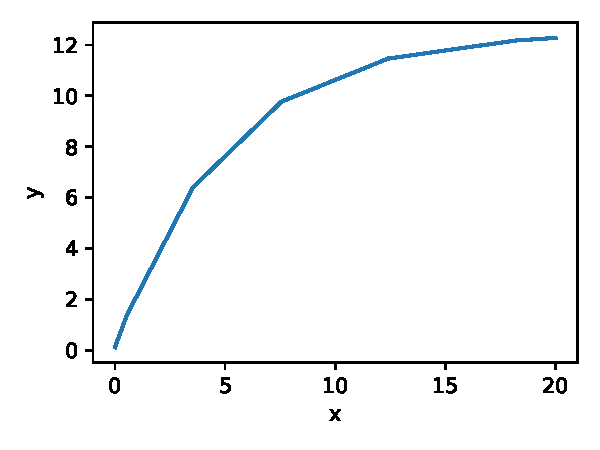
\includegraphics[width=0.7\textwidth]{demo_single_ode.pdf}
      % \begin{tikzpicture}
      %   \begin{axis}[%every axis/.append style={font=\footnotesize},
      %     width=0.95\columnwidth, height=4cm,     % size of the image
      %     grid = major,grid style={dashed, gray!30},
      %     axis background/.style={fill=white},
      %     axis x line=middle,axis y line=middle,ylabel=$y$,xlabel=$x$]
          
      %     \addplot[graph,mark=x] table []{data/ODE_matlabsolve_single2.dat};  
      %     \addlegendentry{$\frac{dy}{dx}$}
      %   \end{axis}
      % \end{tikzpicture}
      % \vfill
    \end{columns}
  \end{itemize}
\end{frame}

\begin{frame}[fragile]
  \frametitle{Solving ODEs in Python: example 2}
  We solve the system: $\displaystyle \frac{dx}{dt} = \begin{cases}
    -\frac{k_1}{x^2} \quad\ \quad t \leq 10\\
    \frac{k_2}{x} - \frac{k_1}{x^2} \quad  t > 10\\
 \end{cases}\, \text{with }\, k_1 = 0.5,\, k_2 = 1,\, x(0) = 2$
 \vspace*{1ex}
  \begin{block}{Create an ODE function}
    \begin{lstlisting}
def myEqnFunction(t,x):
    k1 = 0.5;
    k2 = 1;
    dxdt = int(t>10)*k2/x - k1/x**2;
    return dxdt
    \end{lstlisting}
  \end{block}
  \pause
  \begin{block}{Create a solution script}
    \begin{lstlisting}[backgroundcolor=]x_init = 2;         % Initial condition
tspan = [0, 20]
x_init = [2]
sol = solve_ivp(myEqnFunction, tspan, x_init, rtol=1e-8, atol=1e-6)
    \end{lstlisting}
  \end{block}
\vfill
\end{frame}

{\nologo
\begin{frame}[fragile]
  \frametitle{Solving ODEs in Python: example 2}
  Plot the solution:
  \begin{lstlisting}
plt.plot(sol.t, sol.y[0,:],'r-x')
plt.grid()
plt.show()
  \end{lstlisting}
  \pause
  \begin{center}
    \begin{tikzpicture}
      \begin{axis}[%every axis/.append style={font=\footnotesize},
        width=\textwidth, height=6cm,     % size of the image
        grid = major,grid style={dashed, gray!30},
        axis background/.style={fill=white},
        axis x line=middle,axis y line=middle,ylabel=$x$,xlabel=$t$]

        \addplot[graph,mark=x] table []{data/ODE_matlabsolve_single2.dat};  
        \addlegendentry{$x_1$}
      %  \addlegendentry{$x_2$}
      \end{axis}
    \end{tikzpicture}
  \end{center}
  Note the refinement in regions where large changes occur.
\end{frame}
}

\begin{frame}[label=ode_pass_arguments,fragile]
  \frametitle{Solving ODEs in Python: example}
  A few notes on working with \lstinline$scipy.integrate.solve_ivp$ and other ODE solvers. If we want to give additional arguments (e.g. \lstinline$k1$ and \lstinline$k2$) to our ODE function, we can list them in the function line:
  \begin{lstlisting}
func = lambda t,x,k1,k2: k1*x+k2
# or
def func(t,x,k1,k2):
    return k1*x+k2
  \end{lstlisting}
  The additional arguments can now be set in the solver script by \emph{adding them as \lstinline$args$ list}:
  \begin{lstlisting}
sol = solve_ivp(func,[0,5],[1],args=(k1, k2))
    \end{lstlisting}
  \pause
   Of course, in the solver script, the variables do not have to be called \lstinline$k1$ and \lstinline$k2$:
      \begin{lstlisting}
sol = solve_ivp(func,[0,5],[1],args=(q, u))
    \end{lstlisting}
   These variables may be of any type (scalar, vector, dictionary, list). For carrying over many variables, a dictionary is useful and descriptive.
\end{frame}

\begin{frame}[fragile]
  \frametitle{Solving systems of ODEs in Python: example}
  You have noticed that the step size in $t$ varies. This is because we have given just the begin and end times of our time span:
  \begin{lstlisting}
tspan = [0, 5];
  \end{lstlisting}
  \pause
  You can also obtain the solution at specific points, by supplying a list \lstinline$t_eval$:
  \begin{lstlisting}
sol = solve_ivp(func,tspan,[1],args=(some_k1, some_k2),t_eval=np.linspace(tspan[0],tspan[1],31))
    \end{lstlisting}
  This example provides 31 explicit time steps between 0 and 5 seconds. Note that the results are interpolated to these data points afterwards; you do not influence the efficiency and accuracy of the solver algorithm this way!
  \vfill
\end{frame}